\documentclass[tikz,border=10pt]{standalone}
\usepackage{tikz}
\usetikzlibrary{shapes,arrows,shadows,positioning,fit,backgrounds,calc,matrix}
\usepackage{xcolor}

\definecolor{processblue}{RGB}{52,152,219}
\definecolor{datagreen}{RGB}{46,204,113}
\definecolor{modelorange}{RGB}{230,126,34}
\definecolor{evalred}{RGB}{231,76,60}

\begin{document}
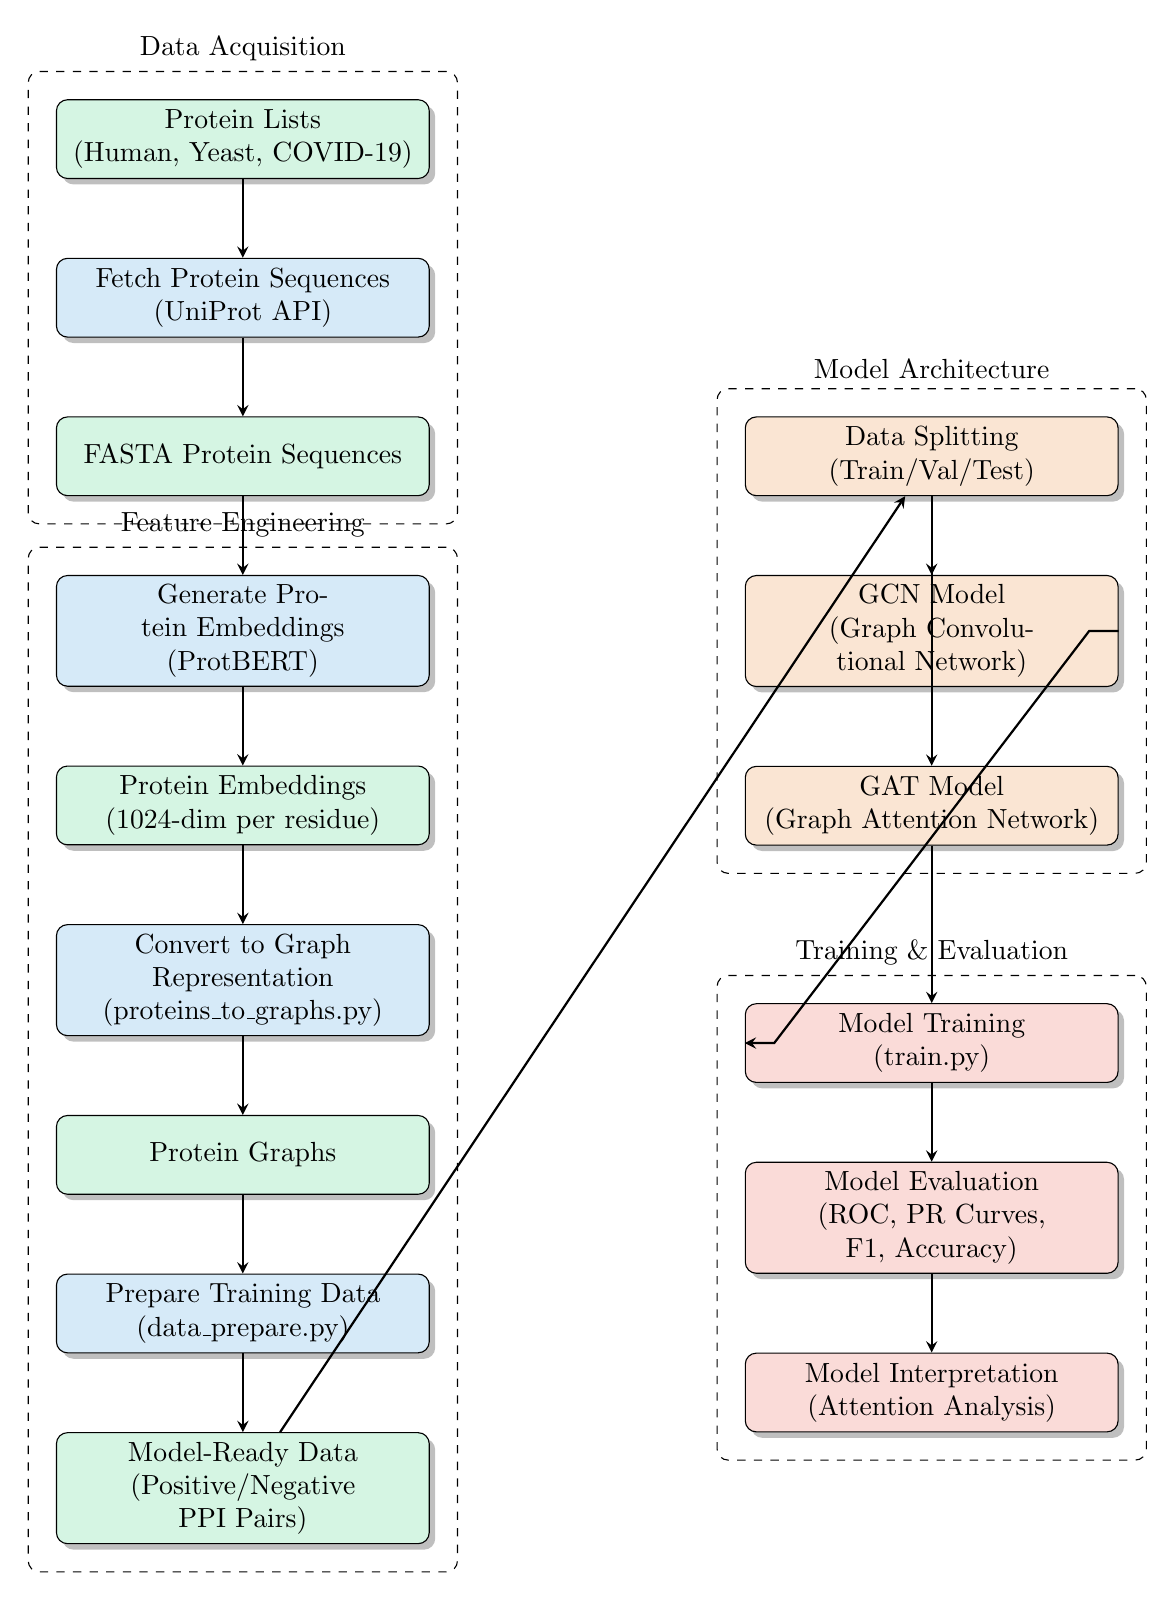
\begin{tikzpicture}[
    node distance=1cm,
    box/.style={draw, rounded corners, fill=white, drop shadow, text width=4.5cm, minimum height=1cm, align=center},
    datanode/.style={box, fill=datagreen!20},
    processnode/.style={box, fill=processblue!20},
    modelnode/.style={box, fill=modelorange!20},
    evalnode/.style={box, fill=evalred!20},
    arrow/.style={thick,->,>=stealth},
    phase/.style={draw, dashed, rounded corners, inner xsep=1em, inner ysep=1em}
]

% Define nodes for Data Acquisition
\node[datanode] (protein_lists) {Protein Lists\\(Human, Yeast, COVID-19)};
\node[processnode, below=of protein_lists] (fetch_sequences) {Fetch Protein Sequences\\(UniProt API)};
\node[datanode, below=of fetch_sequences] (sequences) {FASTA Protein Sequences};

% Define nodes for Data Processing
\node[processnode, below=of sequences] (generate_embeddings) {Generate Protein Embeddings\\(ProtBERT)};
\node[datanode, below=of generate_embeddings] (embeddings) {Protein Embeddings\\(1024-dim per residue)};
\node[processnode, below=of embeddings] (create_graphs) {Convert to Graph Representation\\(proteins\_to\_graphs.py)};
\node[datanode, below=of create_graphs] (protein_graphs) {Protein Graphs};
\node[processnode, below=of protein_graphs] (prepare_data) {Prepare Training Data\\(data\_prepare.py)};
\node[datanode, below=of prepare_data] (model_data) {Model-Ready Data\\(Positive/Negative PPI Pairs)};

% Define nodes for Model Development
\node[modelnode, right=4cm of sequences] (split_data) {Data Splitting\\(Train/Val/Test)};
\node[modelnode, below=of split_data] (gcn_model) {GCN Model\\(Graph Convolutional Network)};
\node[modelnode, below=of gcn_model] (gat_model) {GAT Model\\(Graph Attention Network)};

% Define nodes for Training & Evaluation
\node[evalnode, below=2cm of gat_model] (model_training) {Model Training\\(train.py)};
\node[evalnode, below=of model_training] (model_evaluation) {Model Evaluation\\(ROC, PR Curves, F1, Accuracy)};
\node[evalnode, below=of model_evaluation] (interpret) {Model Interpretation\\(Attention Analysis)};

% Connect everything with arrows
\draw[arrow] (protein_lists) -- (fetch_sequences);
\draw[arrow] (fetch_sequences) -- (sequences);
\draw[arrow] (sequences) -- (generate_embeddings);
\draw[arrow] (generate_embeddings) -- (embeddings);
\draw[arrow] (embeddings) -- (create_graphs);
\draw[arrow] (create_graphs) -- (protein_graphs);
\draw[arrow] (protein_graphs) -- (prepare_data);
\draw[arrow] (prepare_data) -- (model_data);

\draw[arrow] (model_data) -- (split_data);
\draw[arrow] (split_data) -- (gcn_model);
\draw[arrow] (split_data) -- (gat_model);
\draw[arrow] (gcn_model) -- ($(gcn_model)+(2,0)$) -- ($(model_training) + (-2,0)$) -- (model_training);
\draw[arrow] (gat_model) -- (model_training);
\draw[arrow] (model_training) -- (model_evaluation);
\draw[arrow] (model_evaluation) -- (interpret);

% Add phase boxes
\begin{pgfonlayer}{background}
\node[phase, fit=(protein_lists) (sequences), label=above:Data Acquisition] (phase1) {};
\node[phase, fit=(generate_embeddings) (model_data), label=above:Feature Engineering] (phase2) {};
\node[phase, fit=(split_data) (gat_model), label=above:Model Architecture] (phase3) {};
\node[phase, fit=(model_training) (interpret), label=above:Training \& Evaluation] (phase4) {};
\end{pgfonlayer}

\end{tikzpicture}
\end{document}